\documentclass[a4paper]{article}
\usepackage[utf8]{inputenc}
\usepackage[T1]{fontenc}
\usepackage{times}
\usepackage[margin=3cm]{geometry}
\usepackage[english]{babel}

\usepackage[round,authoryear]{natbib}
\usepackage{amsmath,amssymb,amsthm}
\usepackage[hyphens]{url}
\usepackage{graphicx}
\usepackage{booktabs}
\usepackage{xcolor}
\usepackage{tabularx}
\usepackage{tikz}
\usetikzlibrary{arrows.meta,positioning,fit}
\usepackage{pgfplots}
\pgfplotsset{compat=1.18}
\usepackage[most]{tcolorbox}
\usepackage{listings}
\lstset{language=Python, basicstyle=\ttfamily\footnotesize, keywordstyle=\color{blue!60!black},
  commentstyle=\color{green!40!black}\itshape, stringstyle=\color{red!60!black},
  frame=single, rulecolor=\color{gray!50}, backgroundcolor=\color{gray!4},
  columns=fixed, keepspaces=true, showstringspaces=false, breaklines=true,
  xleftmargin=4pt, xrightmargin=4pt, aboveskip=8pt, belowskip=4pt, escapeinside={(*@}{@*)}}
\newcommand{\done}{\textcolor{green!45!black}{\ensuremath{\checkmark}}}
\newcommand{\open}{\textcolor{gray}{\ensuremath{\circ}}}

% Boxes that break up the text: analogies and key points for skimming readers.
\newtcolorbox{analogybox}[1]{enhanced, breakable, colback=blue!4, colframe=blue!45!black,
  fonttitle=\bfseries, title={#1},
  before upper={\setlength{\parskip}{0.6em}\setlength{\parindent}{0pt}}}
\newtcolorbox{keypoints}{enhanced, colback=gray!6, colframe=gray!55!black,
  fonttitle=\bfseries, title={Key points}}
\newtcolorbox{ownview}{enhanced, breakable, colback=green!4, colframe=green!35!black,
  fonttitle=\bfseries, title={My reading},
  before upper={\setlength{\parskip}{0.6em}\setlength{\parindent}{0pt}}}

% Crop a figure from the paper (figures/wang2025-figs.pdf holds pages 2, 7, 9, 13 of the paper).
% \paperfig{page in wang2025-figs}{x0}{y0}{x1}{y1}{width}, coordinates in pt from the top-left corner.
\newcommand{\paperfig}[6]{\includegraphics[page=#1,
  trim={#2pt {\numexpr 792-#5\relax pt} {\numexpr 612-#4\relax pt} #3pt}, clip, width=#6]{figures/wang2025-figs}}

\newtheorem{definition}{Definition}
\newtheorem{theorem}{Theorem}

% Placeholder for text we still have to write. Shown in red in the PDF.
% Remove all \todo{...} before handing in.
\newcommand{\todo}[1]{\textcolor{red}{[TODO: #1]}}


% Link to the supplementary material on OSF (anonymous view-only link).
\newcommand{\supplurl}{\url{https://osf.io/g7qna/files/ed7au?view_only=4862566e18c247a8a43732f0f73118e8}}

% Keep anonymous for the first draft and the peer review; add the name for the final version.
\author{Anonymous (for peer review)}
\title{Can We Trust Membership Inference Attacks to Measure Privacy?}
\date{\today}

\begin{document}

\maketitle

\begin{abstract}
Machine learning models can reveal whether a particular person's data was used to train them, which is itself sensitive when the data comes from, for example, a clinic.
Researchers and auditors measure this risk with membership inference attacks, which try to tell a model's training data apart from other data.
This report explains a recent study showing that these attacks are unreliable as a measuring instrument: repeating the same attack, or switching to a different one, exposes largely different people.
The study also shows that combining several attacks reveals far more of the risk than any single attack.
I explain these findings for readers who are new to the topic, describe my plan to reproduce the study, and report a first test run, which shows that the reproduction is feasible and revealed two errors in the published code.
\end{abstract}


% ---------------------------------------------------------------------------
\section{Introduction}
\label{sec:intro}

Machine learning models do not only learn general patterns from their training data; they can also memorize individual training examples.
A clear demonstration came in 2023, when \citet{nasr2023scalable} spent about 200~USD on queries to ChatGPT (\texttt{gpt-3.5-turbo}) and recovered more than ten thousand examples of its training data word for word, including personal information about dozens of real people.
OpenAI blocked the specific prompt, but variants of the attack kept working until a further fix in early 2024 \citep{breitenbach2024repeated}.

Extracting training data word for word is the most visible form of leakage, but not the only one.
Consider a model trained on patient records from a clinic for the human immunodeficiency virus (HIV).
An attacker who never sees a single record may still be able to tell whether a particular person's record was part of the training data.
For such a dataset, membership alone is sensitive: being in the training set means being a patient of the clinic.
The task of deciding whether a given data point was used to train a model is called \emph{membership inference} \citep{shokri2017membership}.

This risk is not only theoretical.
In 2008, \citet{homer2008resolving} showed that, given a person's genetic profile, a statistical test on the published summary statistics of a genome-wide association study could tell whether that person was among the study participants.
In response, the US National Institutes of Health (NIH) removed such summary data from public databases in August 2008 and made it available only to approved researchers \citep{azbio2008forensic}.
The setting was a statistical study rather than a machine learning model, but the question was the same one a membership inference attack asks.

Because membership is such a direct form of leakage, membership inference attacks (MIAs) have become the standard way to \emph{measure} how much a model reveals about its training data.
They are used to audit models before release, to check whether machine unlearning has really removed a person's data, and to compare privacy defenses \citep{wang2025mia}.
In this role the attack is a measuring instrument rather than a threat: a successful attack signals a high privacy risk, and a failed attack is taken as evidence that the model is safe.

A measuring instrument is only useful if it is reliable.
\citet{wang2025mia} show that MIAs are much less reliable than this use assumes.
Two runs of the same attack that differ only in their random seed flag largely different training points as members.
Different attacks, tuned to the same false positive rate, also disagree about which points are members.
A privacy audit based on a single attack, or on a single run of one, can therefore miss many vulnerable points and underestimate the risk.
The authors propose combining several runs and several attacks into an ensemble; on CIFAR-10, the ensemble detects about five times as many members at a false positive rate of 0.1\% as the best single attack.

This report explains the paper for readers who know the basics of machine learning but have not worked with membership inference before, and describes my plan to reproduce its results.
Section~\ref{sec:background} introduces membership inference, how attacks are evaluated, and the seven attacks the paper studies.
Section~\ref{sec:findings} presents the paper's findings on disparity between attacks and on ensembles.
Section~\ref{sec:reproduction} describes the reproduction plan, the compute it needs, and two bugs I found in the authors' implementation of one attack.
Section~\ref{sec:relwork} places the paper in related work, and Section~\ref{sec:conclusion} concludes.

% ---------------------------------------------------------------------------
\section{Background}
\label{sec:background}

\subsection{What is a membership inference attack?}
\label{subsec:mia}

\begin{analogybox}{An analogy: the ``accidentally'' leaked exam}
A teacher suspects that some students cheat, so they set a trap.
A week before the exam, a copy of half of the exam questions ``accidentally'' ends up on a shared drive.
On exam day, the teacher mixes these leaked questions with new ones that were never on the drive.

Now the teacher does not need to catch anyone opening the file.
A student who read the leak will answer the leaked questions noticeably better, and more confidently, than the new ones of similar difficulty.
An honest student shows no such difference.

A membership inference attack turns this around.
The student is the trained model, and the leaked questions are its training data.
The attacker sees how confidently the model answers a question and decides whether that question was among those it studied.
\end{analogybox}

The analogy also shows what makes the attacker's job hard.
A strong student who understands the material answers new questions almost as well as leaked ones, so the gap is small; in machine learning terms, a model that \emph{generalizes} well leaks less.
And some questions are easy for everyone while others are hard even for students who saw the answer; a fair judgment has to take the difficulty of each question into account.
Both points come back when we look at the individual attacks.

\paragraph{The setting.}
A \emph{target model} $F_T$ is trained on a dataset $D_T$.
The points in $D_T$ are called \emph{members}; points from the same distribution that were not used for training are \emph{non-members}.
Like the paper, we consider \emph{black-box} attacks: the attacker can send an input $x$ to the model and observe its output (for example, the predicted class probabilities), but cannot see the model's weights or its training data.
The attacker also has an \emph{auxiliary dataset} $D_A$ from a similar distribution as $D_T$.

\paragraph{Shadow models.}
Most attacks use $D_A$ to train \emph{shadow models}: models with the same architecture and training procedure as the target, but trained on data the attacker controls.
Because the attacker knows exactly which points each shadow model was trained on, the shadow models show what a member's output looks like compared to a non-member's.
The attack then applies this knowledge to the target model.
Figure~\ref{fig:pipeline} shows the overall structure.

\begin{figure}[!htb]
  \centering
  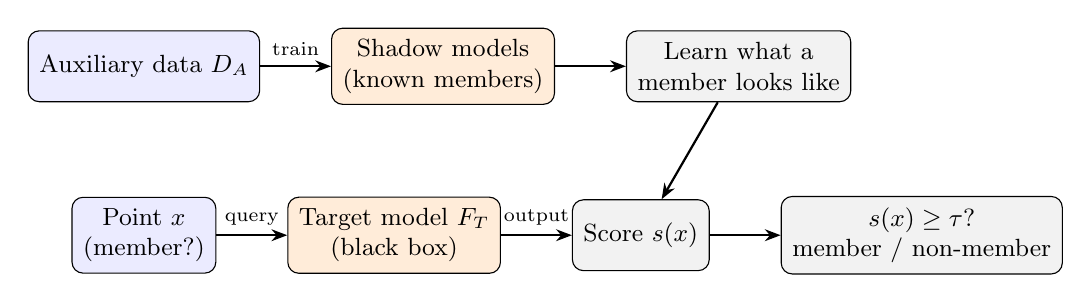
\begin{tikzpicture}[
      node distance=6mm and 9mm,
      box/.style={draw, rounded corners, align=center, minimum height=9mm, inner sep=4pt, font=\small},
      data/.style={box, fill=blue!8},
      model/.style={box, fill=orange!15},
      proc/.style={box, fill=gray!10},
      arr/.style={-{Stealth[length=2mm]}, thick}
    ]
    \node[data]  (aux)    {Auxiliary data $D_A$};
    \node[model, right=of aux]    (shadow) {Shadow models\\(known members)};
    \node[proc,  right=of shadow] (learn)  {Learn what a\\member looks like};

    \node[data,  below=12mm of aux]  (x)      {Point $x$\\(member?)};
    \node[model, right=of x]         (target) {Target model $F_T$\\(black box)};
    \node[proc,  right=of target]    (score)  {Score $s(x)$};
    \node[proc,  right=of score]     (dec)    {$s(x) \geq \tau$?\\member / non-member};

    \draw[arr] (aux) -- node[above, font=\scriptsize]{train} (shadow);
    \draw[arr] (shadow) -- (learn);
    \draw[arr] (x) -- node[above, font=\scriptsize]{query} (target);
    \draw[arr] (target) -- node[above, font=\scriptsize]{output} (score);
    \draw[arr] (learn) -- (score);
    \draw[arr] (score) -- (dec);
  \end{tikzpicture}
  \caption{Structure of a typical membership inference attack. The attacker trains shadow models on auxiliary data to learn how members differ from non-members, then queries the target model with a point $x$, computes a membership score, and compares it with a threshold $\tau$. The simplest attack (LOSS) skips the top row. Own illustration.}
  \label{fig:pipeline}
\end{figure}

Every attack in this report follows the same final step: it computes a \emph{membership score} $s(x)$ for each point and predicts ``member'' if the score exceeds a threshold $\tau$.
The attacks differ in how they compute the score.

\subsection{How attacks are evaluated}
\label{subsec:metrics}

An attack is evaluated on a set of points whose membership is known to the evaluator (half members, half non-members in the paper).
Two numbers describe its predictions at a given threshold, the \emph{true positive rate} (TPR) and the \emph{false positive rate} (FPR):
\[
  \text{TPR} = \frac{\text{members correctly flagged}}{\text{all members}},
  \qquad
  \text{FPR} = \frac{\text{non-members wrongly flagged}}{\text{all non-members}}.
\]
Lowering the threshold flags more points, which raises both rates.
The receiver operating characteristic (ROC) curve plots the TPR against the FPR over all thresholds, and the area under this curve (AUC) summarizes it in one number, where 0.5 means random guessing.

\paragraph{Why AUC is not enough.}
AUC and accuracy are averages over all points.
An attack can reach a respectable AUC by being slightly better than chance on many points, without being confident about any single one.
For privacy, the relevant question is different: can the attacker identify \emph{some} members with high confidence?
\citet{carlini2022membership} therefore argue for reporting the \emph{TPR at a low FPR}, such as 1\% or 0.1\%.
At an FPR of 0.1\%, only one non-member in a thousand is wrongly flagged. If members and non-members are equally common, as in the paper's experiments, even a TPR of 1\% then means that about nine out of ten flagged points are real members. (If members are rare among the tested points, this share drops, so a low FPR alone does not guarantee that the flagged points are members.)
This is the regime that matters in our HIV clinic example: an accusation that is wrong half the time reveals little, one that is almost always right reveals a diagnosis.

Following the paper, we always compare attacks \emph{at the same FPR}: for each attack, the threshold $\tau$ is chosen so that its FPR equals a target value (for example 0.1\%), and the set of points it flags at that threshold is its set of \emph{detected members}.

\paragraph{Comparing sets of detected members.}
The paper's central question is not only \emph{how many} members an attack finds, but \emph{which ones}.
To compare two sets of detected members $A$ and $B$, it uses the \emph{Jaccard index}
\[
  J(A, B) = \frac{|A \cap B|}{|A \cup B|},
\]
which is 1 if both sets are identical and 0 if they share no point.
For example, if one run flags $\{1,2,3,4\}$ and another flags $\{3,4,5,6\}$, then $J = 2/6 \approx 0.33$, although both runs find the same \emph{number} of members.

\subsection{The attacks used in the paper}
\label{subsec:attacks}

The paper studies seven well-known attacks, summarized in Table~\ref{tab:attacks}.
They range from a simple loss threshold to attacks that train dozens of shadow models.
We look at two of them more closely: LOSS, the simplest, and the Likelihood Ratio Attack (LiRA), which is widely regarded as the state of the art.

\begin{table}[!htb]
  \centering
  \small
  \renewcommand{\arraystretch}{1.25}
  \begin{tabularx}{\textwidth}{@{}l X c@{}}
    \toprule
    Attack & Core idea & Shadow models \\
    \midrule
    LOSS \citep{yeom2018privacy} & Members have a lower loss than non-members. One global threshold for all points. & 0 \\
    Class-NN \citep{shokri2017membership} & Train shadow models, then one neural network (NN) classifier per class that learns what the target's output vector looks like for members. & 10 \\
    Augmentation \citep{choquette2021label} & Uses only the predicted labels. Members are still classified correctly when the image is slightly shifted; non-members less often. & 1 \\
    Difficulty calibration \citep{watson2022importance} & Subtract the loss a shadow model has on the same point, so that easy points are not mistaken for members. & 1 \\
    LiRA \citep{carlini2022membership} & For each point, compare the target's loss with the losses of shadow models trained with and without that point. & 20 \\
    Reference \citep{ye2022enhanced} & Compare the target's confidence on a point with that of reference (shadow) models. & 20 (LiRA's) \\
    Loss trajectory \citep{liu2022membership} & Track how the loss of a point changes over training (via distillation), and classify the curve. & 1 \\
    \bottomrule
  \end{tabularx}
  \caption{The seven attacks studied by \citet{wang2025mia}, with the number of shadow models in the paper's setup.}
  \label{tab:attacks}
\end{table}

\paragraph{LOSS: one threshold for everyone.}
The LOSS attack \citep{yeom2018privacy} uses the most direct signal: a model's loss is usually lower on points it was trained on.
It flags a point as a member if the target model's loss on it is below a single global threshold.
LOSS needs no shadow models and involves no randomness, so running it twice always gives the same result, which will make it a useful baseline in Section~\ref{sec:findings}.
Its weakness is the one the exam analogy pointed out: a global threshold ignores difficulty.
An easy non-member has a low loss and is wrongly flagged, while a hard or unusual member keeps a high loss and is missed (Figure~\ref{fig:loss-vs-lira}, left).

\paragraph{LiRA: a separate test for every point.}
LiRA \citep{carlini2022membership} fixes this by judging each point against its own baseline.
The attacker puts $D_A$ and the points to be tested into one pool and trains many shadow models, each on a random half of this pool, so that every tested point $x$ was in the training set of some shadow models (``IN'') and not in others (``OUT'').
For each point, LiRA collects the shadow models' losses on $x$ and fits two Gaussian (normal) distributions, one to the IN losses and one to the OUT losses, with means $\mu_{\text{in}}, \mu_{\text{out}}$ and variances $\sigma_{\text{in}}^2, \sigma_{\text{out}}^2$.
It then asks which of the two better explains the loss $\ell_T(x)$ of the target model, by comparing the two Gaussian densities $\mathcal{N}$ at this loss:
\[
  s_{\text{LiRA}}(x) = \frac{\mathcal{N}\!\left(\ell_T(x);\, \mu_{\text{in}}, \sigma_{\text{in}}^2\right)}{\mathcal{N}\!\left(\ell_T(x);\, \mu_{\text{out}}, \sigma_{\text{out}}^2\right)}.
\]
A score well above 1 means the target behaves on $x$ like a model that was trained on it (Figure~\ref{fig:loss-vs-lira}, right).
(Strictly speaking, LiRA does not use the loss itself but a rescaled form of the model's confidence $p$ in the correct label, $\log\frac{p}{1-p}$. It carries the same information, since a lower loss means a higher confidence, but is closer to a normal distribution.)
Because the test adapts to each point, LiRA finds members that a global threshold misses, especially at low FPR.
The price is compute: in the paper's setup, LiRA trains 20 shadow models per run, which makes it by far the most expensive attack (Section~\ref{subsec:budget}).
The random split of the pool for each shadow model is also a source of randomness, so two runs of LiRA do not flag exactly the same points; this is the starting point of Section~\ref{sec:findings}.

\begin{figure}[t]
  \centering
  \pgfmathdeclarefunction{gauss}{3}{\pgfmathparse{1/(#3*sqrt(2*pi))*exp(-((#1-#2)^2)/(2*#3^2))}}
  \begin{tikzpicture}
    \begin{axis}[
        name=left, width=0.5\textwidth, height=4.6cm,
        domain=0:3.5, samples=120, axis lines=left,
        xlabel={loss}, ylabel={density}, ytick=\empty, xtick=\empty,
        ymin=0, ymax=1.75, title={\small LOSS: all points, one threshold},
        legend style={font=\scriptsize, draw=none, fill=none, at={(0.98,0.98)}, anchor=north east}]
      \addplot[blue!70!black, thick] {gauss(x,0.6,0.35)};
      \addlegendentry{members}
      \addplot[red!70!black, thick, dashed] {gauss(x,1.7,0.55)};
      \addlegendentry{non-members}
      \addplot[fill=red!25, draw=none, domain=0:1.0, forget plot] {gauss(x,1.7,0.55)} \closedcycle;
      \draw[thick] (axis cs:1.0,0) -- (axis cs:1.0,1.3) node[above, font=\scriptsize] {$\tau$};
      \node[font=\scriptsize, align=center] at (axis cs:0.5,1.5) {flagged\\[-2pt]$\leftarrow$};
    \end{axis}
    \begin{axis}[
        at={(left.east)}, anchor=west, xshift=1.2cm,
        width=0.5\textwidth, height=4.6cm,
        domain=0:3.5, samples=120, axis lines=left,
        xlabel={loss on one point $x$}, ytick=\empty, xtick=\empty,
        ymin=0, ymax=1.75, title={\small LiRA: one point, IN vs.\ OUT},
        legend style={font=\scriptsize, draw=none, fill=none, at={(0.98,0.98)}, anchor=north east}]
      \addplot[blue!70!black, thick] {gauss(x,1.3,0.3)};
      \addlegendentry{IN shadows}
      \addplot[red!70!black, thick, dashed] {gauss(x,2.4,0.35)};
      \addlegendentry{OUT shadows}
      \draw[thick, -{Stealth}] (axis cs:1.45,1.5) -- (axis cs:1.45,0.02);
      \node[font=\scriptsize, align=center, anchor=south] at (axis cs:1.45,1.5) {$\ell_T(x)$};
    \end{axis}
  \end{tikzpicture}
  \caption{Schematic, not real data. Left: LOSS uses one threshold $\tau$ for all points. Non-members with a low loss (shaded) are wrongly flagged, and members with a high loss are missed. Right: LiRA looks at a single, hard point $x$. Its loss is high even for models trained on it, so LOSS would not flag it, but the target's loss $\ell_T(x)$ matches the IN distribution much better than the OUT distribution, so LiRA does. Own illustration.}
  \label{fig:loss-vs-lira}
\end{figure}

\begin{keypoints}
\begin{itemize}
  \item A membership inference attack computes a score for each point and flags it as a member if the score exceeds a threshold.
  \item Most attacks train \emph{shadow models} on auxiliary data to learn what members look like. This training is random.
  \item The meaningful measure is the TPR at a low FPR (e.g.\ 0.1\%): how many members an attack finds while almost never accusing a non-member.
  \item The paper compares attacks at the same FPR and asks which members they find; the Jaccard index measures how much two sets of detected members overlap.
\end{itemize}
\end{keypoints}

% ---------------------------------------------------------------------------
\section{What the paper finds}
\label{sec:findings}

The paper asks whether the usual way of using MIAs as a privacy tool is sound: pick the attack with the best scores (AUC, accuracy, TPR at low FPR), run it once, and report the result \citep{wang2025mia}.
It approaches the question from two sides.
First, does a single attack give the same answer when it is run again with a different random seed (\emph{instance-level disparity})?
Second, do different attacks find the same members (\emph{method-level disparity})?
The answer to both is largely no, and the paper turns this into an ensemble that finds many more members than any single attack.

Most experiments use CIFAR-10 with a ResNet-56 target model, and six runs (``instances'') per attack.
One detail is easy to miss: unless stated otherwise, the paper sets each attack's threshold to an FPR of 0.1, which means \emph{10\%}, not 0.1\%.
The disparity results below are therefore measured at a fairly generous false positive rate; only the ensemble results in Section~\ref{subsec:ensemble} use the strict 0.1\%.

\subsection{Same attack, different runs: instance-level disparity}
\label{subsec:instance-disparity}

Every attack except LOSS involves randomness: how the auxiliary data is split for the shadow models, how their weights are initialized, the order of the training batches, and the training of any attack classifier.
The paper fixes all of this with a single random seed and treats each seed as one \emph{instance} of the attack, the version that one particular attacker might end up with.
All instances use the same auxiliary data and attack the same target model.

Figure~\ref{fig:paper-venn}(b) shows the result for three instances of Class-NN.
Each circle is the set of members one instance detects, and the circles overlap far less than one would expect from ``the same attack''.
Only 424 members (14.6\% of those found by any of the three) are found by all three runs.

\begin{figure}[!htb]
  \centering
  \paperfig{1}{53}{70}{298}{224}{0.62\textwidth}
  \caption{Members detected on CIFAR-10 at what the paper calls a ``low FPR (0.1)''.\protect\footnotemark{} (a)~Three different attacks: LiRA, Loss trajectory and Reference. (b)~Three instances of the same attack (Class-NN), differing only in their random seed. Reproduced from \citet[Fig.~1]{wang2025mia}.}
  \label{fig:paper-venn}
\end{figure}
\footnotetext{The member counts in this figure are much smaller than in the paper's other results at an FPR of 10\%, so this figure may use a stricter FPR. I will check this in the reproduction.}

\paragraph{Consistency.}
To put a number on this, the paper defines the \emph{consistency} of an attack as the average Jaccard index (Section~\ref{subsec:metrics}) between the detected members of every pair of instances.
A consistency of 1 means every run finds exactly the same members.
LOSS, which has no randomness, always scores 1.
Every other attack scores low: averaged over datasets and architectures, consistency stays below 0.4 (Figure~\ref{fig:paper-consistency}).
Consistency is somewhat higher on CIFAR-100, where target models overfit more and so more members are easy to detect.
Class-NN is the least consistent, which the authors attribute to its shadow models being trained on disjoint parts of $D_A$.

\begin{figure}[!htb]
  \centering
  \paperfig{2}{53}{70}{222}{203}{0.5\textwidth}
  \caption{Consistency of each attack on CIFAR-10, measured over six instances at an FPR of 10\%, for four target architectures. Only LOSS reaches 1. Reproduced from \citet[Fig.~4a]{wang2025mia}.}
  \label{fig:paper-consistency}
\end{figure}

\paragraph{Coverage and stability.}
If different runs find different members, which set is ``the'' result of an attack?
The paper uses two answers.
The \emph{coverage} of an attack is the union of the true positives of all its instances: every member that \emph{some} run detects.
The \emph{stability} is the intersection: the members that \emph{every} run detects.
Coverage describes how far an attack's reach extends, and stability describes the members it finds reliably.

The two behave very differently as more instances are added.
With 16 instances, the coverage of the best attacks grows to a TPR of about 0.69, but its FPR grows as well, to as much as 0.60, because each run also brings its own false positives.
The stability shrinks to a TPR of about 0.10 or less, but its FPR drops to almost zero (except for LOSS, which does not change), so the few members that remain are nearly all real: for Loss trajectory, Calibration and LiRA, more than 95\% of the points in their stability set are members.
Both sets settle down after about six instances, which is why the paper uses six.

\begin{ownview}
Why would the same attack find different members each time? I find it helpful to think about where a point's score sits relative to the threshold.
A few members are so clearly memorized that their score is far above the threshold in every run; these form the stability set.
Many more members score only slightly above the typical non-member, and for them the noise from the shadow models decides which side of the threshold they land on. At a fixed FPR, each run has the same ``budget'' of false positives, so the threshold sits right in this crowded region, and small changes in the scores shuffle which points get flagged.

A rough baseline puts the numbers in context. If two runs each flagged a random 25\% of the members (roughly the TPR the attacks reach at 10\% FPR), their expected Jaccard index would be $0.25/(2-0.25) \approx 0.14$. The measured consistencies of about 0.2--0.4 are above this, so the runs do agree on a common core, but they are much closer to independent guesses than to a deterministic measurement.
\end{ownview}

\subsection{Different attacks: method-level disparity}
\label{subsec:method-disparity}

The second question is whether different attacks find the same members.
Comparing single instances would mix this question with the randomness from Section~\ref{subsec:instance-disparity}, so the paper compares the coverage and the stability of each pair of attacks, each computed from six instances, using the Jaccard index.

Figure~\ref{fig:paper-venn}(a) gives a first impression: of the roughly 1{,}250 members that LiRA, Loss trajectory and Reference detect between them, only 26 are found by all three, and more than 40\% are found by Loss trajectory alone.
Figure~\ref{fig:paper-jaccard} shows the full comparison.
For coverage, most pairs of attacks have a Jaccard index below 0.4.
For stability, the values are mostly below 0.1: the members that each attack finds \emph{reliably} are almost entirely different from attack to attack.
The most similar pairs are the ones that share ingredients, such as LiRA and Reference, which use the same 20 shadow models, and the three attacks based on the loss (Calibration, Loss trajectory and Reference).
LOSS has a low similarity with everything else.

The paper also repeats the comparison at FPRs from 0.1\% to 20\% and finds that the similarity \emph{decreases} as the FPR gets stricter.
In other words, the members an attack is most confident about, which are exactly the ones that matter in the low-FPR regime, are the ones on which attacks disagree most.

\begin{figure}[!htb]
  \centering
  \paperfig{3}{53}{70}{298}{207}{0.8\textwidth}
  \caption{Jaccard index between the (a)~coverage and (b)~stability of each pair of attacks, averaged over four experiment runs; CIFAR-10, six instances per attack, FPR of 10\%. Reproduced from \citet[Fig.~10]{wang2025mia}.}
  \label{fig:paper-jaccard}
\end{figure}

\begin{analogybox}{Back to the leaked exam}
Suppose several teachers try to catch the students who read the leaked exam, each with their own method.
One compares scores on leaked and new questions, one looks at how quickly a student answered, and one checks whether wrong answers match a typo in the leaked copy.
Each method catches the cheaters who give themselves away in \emph{that} particular way, so each teacher ends up with a different list.
None of the lists is wrong, but a school that trusted only one teacher would believe it had fewer cheaters than it really has.
\end{analogybox}

\subsection{Why the disparity happens}
\label{subsec:why-disparity}

The paper tests which parts of an attack's randomness cause the instance-level disparity (Figure~\ref{fig:paper-factors}).

\begin{itemize}
  \item \textbf{Shadow model training.} Giving all instances the same initial weights for their shadow models changes consistency by at most 0.05. The main cause is therefore not the weights but how the data is split and shuffled when the shadow models are trained.
  \item \textbf{Attack model training.} For attacks with a learned attack classifier (Class-NN, Augmentation, Loss trajectory), fixing the shadow models so that every instance trains its classifier on the same data raises consistency by only 8--12\%. The classifier training adds some disparity, but less than the shadow models.
  \item \textbf{Number of shadow models.} More shadow models raise consistency slightly, most clearly for Calibration, whose difficulty estimate becomes less noisy. Even with 100 shadow models for LiRA and Reference, the disparity remains large.
\end{itemize}

\begin{figure}[!htb]
  \centering
  \paperfig{2}{53}{240}{298}{359}{0.65\textwidth}
  \caption{Effect of (a)~the shadow models' initial weights and (b)~a fixed attack training set on consistency (CIFAR-10, six instances, FPR of 10\%). ``True'' means the factor is varied between instances in (a), and fixed in (b). Reproduced from \citet[Fig.~5]{wang2025mia}.}
  \label{fig:paper-factors}
\end{figure}

For the method-level disparity, the paper offers a first, partly exploratory explanation.
Different attacks use different \emph{signals}: a single loss value, the full output vector, the output on shifted images, or a loss trajectory over training.
Each signal makes some members stand out and hides others.
Looking at the target model's outputs on the members that only one attack detects, the authors find that these members form visibly different groups for different attacks, so each attack seems to favor a particular kind of member.

\subsection{Ensembles of attacks}
\label{subsec:ensemble}

The two kinds of disparity suggest a simple fix: if every run and every attack sees a different part of the picture, combine them.
The paper's ensemble works in two steps (Figure~\ref{fig:ensemble}):
\begin{enumerate}
  \item \textbf{Within each attack}, combine its six instances into one prediction, in one of three ways: \emph{stability} (a point is a member only if all instances agree, logical AND), \emph{coverage} (if any instance says so, logical OR), or \emph{majority vote}.
  \item \textbf{Across attacks}, take the union (logical OR) of the combined predictions.
\end{enumerate}
Combining predictions changes the FPR: a union of several attacks has more false positives than each attack alone. The paper therefore does not fix the single instances at one FPR. It repeats the ensemble for 100 different FPR settings of the single instances, measures the TPR and FPR of the ensemble's final prediction each time, and so obtains the ensemble's own ROC curve. The ensemble's TPR at 0.1\% FPR and its AUC are taken from this curve, so the comparison with single attacks is at the same FPR.
The ensemble uses four attacks: LiRA, Reference, Loss trajectory and Calibration.
These are the four whose precision clearly improves when their instances are combined by stability; Class-NN and Augmentation do not show this effect, and LOSS has no randomness to average out.

\begin{figure}[!htb]
  \centering
  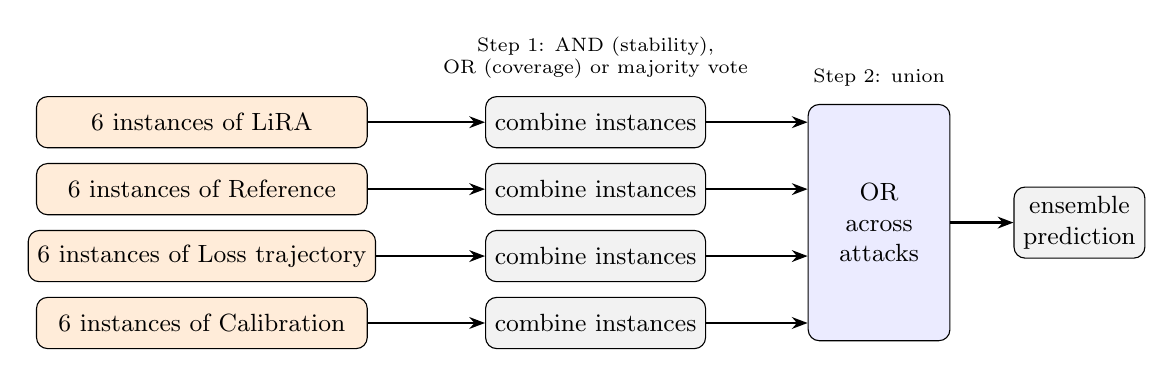
\begin{tikzpicture}[
      runs/.style={draw, rounded corners, fill=orange!15, minimum width=42mm, minimum height=6.5mm, font=\small},
      comb/.style={draw, rounded corners, fill=gray!10, minimum width=26mm, minimum height=6.5mm, font=\small},
      arr/.style={-{Stealth[length=2mm]}, thick}
    ]
    \foreach \a [count=\i] in {LiRA, Reference, Loss trajectory, Calibration} {
      \node[runs] (r\i) at (0,-0.85*\i) {6 instances of \a};
      \node[comb] (c\i) at (5.0,-0.85*\i) {combine instances};
      \draw[arr] (r\i) -- (c\i);
    }
    \node[draw, rounded corners, fill=blue!8, minimum height=30mm, minimum width=18mm, align=center, font=\small]
      (or) at (8.6,-2.125) {OR\\across\\attacks};
    \foreach \i in {1,...,4} \draw[arr] (c\i.east) -- (or.west |- c\i);
    \node[draw, rounded corners, fill=gray!10, align=center, font=\small, right=8mm of or] (out) {ensemble\\prediction};
    \draw[arr] (or) -- (out);
    \node[font=\scriptsize, align=center, above=1mm of c1] {Step 1: AND (stability),\\OR (coverage) or majority vote};
    \node[font=\scriptsize, align=center, above=1mm of or] {Step 2: union};
  \end{tikzpicture}
  \caption{The two-step ensemble of \citet{wang2025mia}. Own illustration; the paper describes the procedure only in text and formulas.}
  \label{fig:ensemble}
\end{figure}

The stability and majority-vote ensembles work best at low FPR, and the reason follows directly from the previous sections.
Step~1 removes the noise of individual runs: requiring agreement removes the points that were flagged by chance and keeps each attack's reliable core, which has very few false positives.
Step~2 then benefits from the method-level disparity: because the reliable cores of different attacks hardly overlap (Figure~\ref{fig:paper-jaccard}b), their union contains many more members, while the false positives stay few.
What looked like a weakness of MIAs, that they disagree, is what makes the ensemble strong.

Table~\ref{tab:ensemble} shows the gain.
On CIFAR-10, the best single instance (Reference) detects 1.0\% of members at an FPR of 0.1\%; the majority-vote ensemble detects 5.6\%, and the stability ensemble 5.0\%.
On CIFAR-100, the stability ensemble raises the TPR from 4.2\% to 28\%.
Figure~\ref{fig:paper-roc} shows that the ensembles stay above the single instances across the whole range of FPRs.
The gain comes at a price: the full ensemble needs six instances of four attacks.
The paper notes that this can be reduced, for example because LiRA and Reference can share their shadow models, and that three instances per attack already reach a similar TPR at roughly half the cost.

\begin{table}[!htb]
  \centering
  \small
  \begin{tabular}{@{}llcccc@{}}
    \toprule
    & & \multicolumn{2}{c}{CIFAR-10} & \multicolumn{2}{c}{CIFAR-100} \\
    \cmidrule(lr){3-4} \cmidrule(l){5-6}
    & Attack / strategy & AUC & TPR@0.1\% & AUC & TPR@0.1\% \\
    \midrule
    Single instance & Loss trajectory & 0.635 & 0.002 & 0.852 & 0.042 \\
                    & Reference       & 0.608 & 0.010 & 0.813 & 0.034 \\
                    & LiRA            & 0.585 & 0.005 & 0.802 & 0.034 \\
                    & Calibration     & 0.603 & 0.005 & 0.721 & 0.008 \\
    \midrule
    Ensemble        & Coverage        & 0.841 & 0.025 & 0.913 & 0.077 \\
                    & Stability       & \textbf{0.863} & 0.050 & \textbf{0.978} & \textbf{0.280} \\
                    & Majority vote   & 0.858 & \textbf{0.056} & 0.961 & 0.208 \\
    \bottomrule
  \end{tabular}
  \caption{Single instances against the full four-attack ensembles (ResNet-56). Values from \citet[Table~1]{wang2025mia}, which also reports CINIC-10 and accuracy.}
  \label{tab:ensemble}
\end{table}

\begin{figure}[!htb]
  \centering
  \paperfig{4}{53}{70}{559}{200}{\textwidth}
  \caption{ROC curves (log scale) of the (a)~stability, (b)~coverage and (c)~majority-vote ensembles on CIFAR-10. Dashed: single instances; solid: one attack's instances combined; black: the full four-attack ensemble. Reproduced from \citet[Fig.~15]{wang2025mia}.}
  \label{fig:paper-roc}
\end{figure}

\begin{ownview}
Two observations help me read these results correctly.
First, the ensemble is not a new way of extracting information from the model; it only combines the predictions of existing attacks. That it finds five times as many members means that each single attack was leaving most of the vulnerable members undetected.

Second, the ensemble is a realistic model of the threat. An attacker is not limited to one run of one attack, and different attackers will use different methods and seeds. Judging a model by one instance therefore measures the risk from one particular attacker, not the risk the model is exposed to.
\end{ownview}

\subsection{What this means for privacy in practice}
\label{subsec:implications}

When an MIA is used as a privacy tool, the reasoning usually goes: ``the attack found few members, so the model leaks little''.
But an attack can only show that leakage \emph{exists}, so its result is a lower bound on the risk, and disparity makes the lower bound from one run of one attack loose.
The paper names three common uses where this matters:
\begin{itemize}
  \item \textbf{Privacy auditing.} Auditing tools often run one instance of each attack and report average metrics, so the vulnerable members that this instance misses go unreported.
  \item \textbf{Machine unlearning.} To check that a model has ``forgotten'' some data, papers test whether one MIA instance can still detect it. Another instance may still detect it.
  \item \textbf{Evaluating defenses.} A defense tested against one instance is only shown to protect the members that this instance exposes.
\end{itemize}
The paper therefore recommends reporting results over several instances and several attacks, and including an ensemble in the evaluation.
For our HIV clinic example, a single failed attack is not evidence that a patient's membership is safe.

\begin{keypoints}
\begin{itemize}
  \item The same attack run with different random seeds flags largely different members; only LOSS is consistent. The main cause is the random data splits used to train shadow models.
  \item Different attacks also flag different members, and they disagree most about the members they are most confident about.
  \item Combining instances (to remove noise) and then attacks (to collect their different findings) detects about five times more members at 0.1\% FPR on CIFAR-10 than the best single instance.
  \item A privacy evaluation based on one run of one attack underestimates the risk.
\end{itemize}
\end{keypoints}

% ---------------------------------------------------------------------------
\section{Reproduction plan}
\label{sec:reproduction}

The paper's conclusions rest entirely on experiments, so the most direct way to check them is to repeat those experiments.
The goal of my reproduction is the \emph{whole} paper: every figure and table in the main text, and the appendix experiments they depend on.
After discussion with my supervisor, the only reduction we allow is in the number of shadow-model settings for the experiment in \citet[Fig.~6]{wang2025mia}, which at full size would cost about a quarter of the total budget (Section~\ref{subsec:budget}).

\subsection{Setup}
\label{subsec:setup}

The authors published their code, which implements all seven attacks, the experiment scripts and the analysis notebooks.%
\footnote{\url{https://github.com/RPI-DSPlab/mia-disparity}, checked at commit \texttt{71a2965} (January 2026).}
I use it as published and record every change I make, so that each result can be traced back to the authors' code or to a documented change.
As an independent check, I also compute the central quantities (consistency, coverage, stability and the stability ensemble) with my own short implementation.

I follow the paper's setup \citep[Sec.~4.1 and App.~A]{wang2025mia}.
The datasets are CIFAR-10, CIFAR-100 and CINIC-10 (images) and Purchase-100 and Texas-100 (tabular).
Each image dataset is split into a target set of 30{,}000 points (15{,}000 members and 15{,}000 non-members) and a separate auxiliary set of 30{,}000 points for the attacker.
The target models are ResNet-56, WideResNet-32-4, VGG-16 and MobileNetV2 for images, and a small multilayer perceptron (MLP) for the tabular data.
As in the paper, ResNet-56 on CIFAR-10 is the main setting.

I develop and test on my laptop, which has an Nvidia RTX 5070 graphics processing unit (GPU) with 8\,GB of memory.
The full reproduction runs on sciCORE, the computing cluster of the University of Basel.
The main setting runs on Nvidia L40S GPUs, the model on which the paper reports its run times \citep[extended version, App.~C.1]{wang2025mia}, so the times can be compared directly; the other experiments run on A100 GPUs.
The laptop's GPU is too new for the version of the PyTorch library that the code requires, so on the laptop I use a current version, which needed two small changes (Section~\ref{subsec:issues}).

\subsection{Experiments, stages and budget}
\label{subsec:budget}

Table~\ref{tab:experiments} lists the experiments needed for the full paper and the results each one reproduces.
A \emph{seed set} is one run of all seven attacks for one dataset, model and random seed.
Most results need six seeds (instances) per attack, and the convergence curves need 16 \citep[Figs.~7--9]{wang2025mia}.
The cost is given in GPU-hours (GPU-h): one hour of computation on one GPU.

\begin{table}[!htb]
  \centering
  \small
  \renewcommand{\arraystretch}{1.2}
  \begin{tabularx}{\textwidth}{@{}l X l r@{}}
    \toprule
    & Experiment & Paper results & GPU-h \\
    \midrule
    S & Data splits and target models & prerequisite & 15 \\
    A & Main grid: 3 image datasets $\times$ 4 models $\times$ seeds 0--5 (72 seed sets) & Figs.~1, 2, 4, 10--12, 15--17; Table~1 & 1{,}350 \\
    B & 10 extra seeds for CIFAR-10 and CIFAR-100 (ResNet-56) & Figs.~7--9 (16 instances) & 310 \\
    C & 3 more random data partitions (CIFAR-10, CIFAR-100) & Fig.~10 (``average of 4 runs'') & 560 \\
    D & Tabular data: Purchase-100, Texas-100 & appendix & 6 \\
    E & Same initial weights; same attack training set & Fig.~5 & 75 \\
    F & Number of shadow models (reduced, see below) & Fig.~6 & 500 \\
    G & Class-NN with top-1/3/10 outputs only & Fig.~13 & 9 \\
    H & Offline LiRA & appendix & 6 \\
    I & Gap between auxiliary and target data & appendix & 5 \\
    \midrule
    & \textbf{Total} (about 520 GPU jobs) & & \textbf{2{,}850} \\
    \bottomrule
  \end{tabularx}
  \caption{Experiments for the full reproduction, with estimated cost in L40S GPU-hours (rounded). Paper results refer to \citet{wang2025mia}.}
  \label{tab:experiments}
\end{table}

The estimates start from the paper's run times for one instance on CIFAR-10/ResNet-56 on an L40S \citep[extended version, App.~C.1]{wang2025mia}.
LiRA dominates with 580 minutes, 540 of which are spent training its 20 shadow models.
Reference reuses these shadow models, and Loss trajectory and Calibration take only 17 and 5 minutes.
With my estimates for the other attacks, \textbf{one seed set costs about 11.7 GPU-hours}.
I scale this by the number of training epochs and the model size for the other settings and add a 15\% margin for failed runs, which gives about \textbf{3{,}300 GPU-hours} in total.
The most expensive single experiment is Fig.~6 of the paper, which varies the number of shadow models from 20 to 100.
Each setting needs its own shadow models, so I test only 20, 60 and 100 (and 1, 3, 7 and 13 for Calibration), which keeps both ends of the curve and saves about 350 GPU-hours.
With up to 24 GPUs at once, the whole plan takes about six days of computation, or two to four weeks with realistic waiting times on the cluster.

The work runs in stages, so that problems appear while they are still easy to fix:
\begin{enumerate}
  \item \textbf{Smoke test} on the laptop with very short training, to check that the code runs (Section~\ref{subsec:smoke}).
  \item \textbf{Pilot} on the cluster (about 25 GPU-hours), whose measured times replace my estimates.
  \item \textbf{Main setting} (CIFAR-10/ResNet-56, six seeds, about 70 GPU-hours), which already covers the paper's central results: Figures~\ref{fig:paper-venn}--\ref{fig:paper-jaccard} and~\ref{fig:paper-roc}, and the CIFAR-10 column of Table~\ref{tab:ensemble}.
  \item \textbf{Full grid} of Table~\ref{tab:experiments}, followed by the \textbf{analysis}: recreating every figure and table, checking the central numbers with my own code, and comparing them with the paper.
\end{enumerate}

\subsection{Issues found in the code so far}
\label{subsec:issues}

Reading the code and running the smoke test revealed three kinds of issues: problems that stop the code from running but do not affect results, gaps where the published code is incomplete, and two bugs in the Augmentation attack that do change its results.

\paragraph{Fixes that do not change results.}
Table~\ref{tab:fixes} lists the changes I made so that the code runs.
None of them changes what the code computes; for the memory fix, I verified that the output is identical.

\begin{table}[!htb]
  \centering
  \small
  \renewcommand{\arraystretch}{1.2}
  \begin{tabularx}{\textwidth}{@{}l X X@{}}
    \toprule
    Where & Problem & Change \\
    \midrule
    Augmentation attack & Shifting all images in one call needs about 34\,GB of memory for the 30{,}000 target images, more than my laptop has. & Shift in chunks of 1{,}000 images. Output identical (maximum difference 0.0). \\
    Newer PyTorch & One function the code uses no longer exists, and whole saved models are no longer loaded by default. & Python's \texttt{itertools.accumulate}, which gives the same split, and the setting \texttt{TORCH\_\allowbreak FORCE\_\allowbreak NO\_\allowbreak WEIGHTS\_\allowbreak ONLY\_\allowbreak LOAD=1}. \\
    Experiment scripts & Placeholder data paths, a fixed second GPU, all seeds launched in parallel on one GPU, and a crash in the data preparation that the script hid by continuing after errors. & Settings via environment variables (with the paper's values as defaults), seeds one after another, the faulty check skipped, and a stop at the first error. \\
    \bottomrule
  \end{tabularx}
  \caption{Changes needed to run the published code. None of them affects the results.}
  \label{tab:fixes}
\end{table}

\paragraph{Gaps in the published code.}
Some experiments cannot be run from the repository as it is.
A file needed for the accuracy tables (\texttt{obtain\_accuracy.py}) is missing, there is no code for the two setups of Fig.~5, and the experiment on the gap between auxiliary and target data is not documented.
The number of shadow models and the number of top classes that Class-NN sees in Fig.~13 are fixed in the code.
I will ask the authors for the missing pieces and report any remaining guesses about their setup.

\paragraph{Bug 1: mismatched class labels in the Augmentation attack.}
The Augmentation attack \citep{choquette2021label} trains one attack classifier per class.
To build its training data, it splits the auxiliary data into a shadow training set (members) and a test set (non-members), computes the shadow model's features for each point, and attaches each point's class label.
The features and the labels, however, come out in different orders (simplified from \texttt{miae/attacks/aug\_mia.py}):

\begin{lstlisting}
trainloader = DataLoader(train_set, ..., shuffle=True)   # (*@\textbf{random order}@*)
testloader  = DataLoader(test_set,  ..., shuffle=False)

aug_in  = augmentation_process(shadow_model, train_set)  # features, dataset order
aug_out = augmentation_process(shadow_model, test_set)

for _, target in trainloader:     # labels of the members, in (*@\textbf{shuffled}@*) order
    in_labels = concatenate(in_labels, target)
for _, target in testloader:      # labels of the non-members, in dataset order
    out_labels = concatenate(out_labels, target)

attack_features = concatenate(aug_in, aug_out)
attack_labels   = concatenate(in_labels, out_labels)   # row i of in_labels does not
                                                       # belong to row i of aug_in
\end{lstlisting}

Because the shadow training loader shuffles, the $i$-th member label belongs to a random point, not to the $i$-th member's features.
The non-member labels are correct, since their loader does not shuffle.
As a result, the attack classifier for class $j$ is trained on non-members of class $j$ but on members of \emph{random} classes, so it does not learn what a member of class $j$ looks like, which is the idea of the per-class design.
The fix is to take the labels from the dataset in its original order.

\paragraph{Bug 2: the ``translations'' shift the wrong axes.}
The attack's signal is whether the model still classifies an image correctly when it is moved by a few pixels.
The code creates nine shifts and applies them with \texttt{scipy.ndimage.shift}, which takes one displacement per array axis:

\begin{lstlisting}
AugUtil.create_translates(2)
# -> [(0,0,0,0), (0,2,0,0), (0,1,-1,0), (0,0,-2,0), (0,-1,-1,0),
#     (0,-2,0,0), (0,-1,1,0), (0,0,2,0), (0,1,1,0)]

x, y = get_xy_from_dataset(data)        # x.shape == (N, 3, 32, 32): (N, C, H, W)
shift(x, (0, 2, 0, 0), mode='nearest')  # intended: move 2 pixels down
                                        # actual: shift along the color channels
\end{lstlisting}

The shifts have the form $(0, d_y, d_x, 0)$, where $d_y$ and $d_x$ are the intended vertical and horizontal displacements in pixels. This is correct for images stored as (images, height, width, channels).
The function's own documentation asks for this layout, which is presumably carried over from the TensorFlow implementation of the original attack.
In PyTorch, however, images are stored as (images, channels, height, width).
The ``vertical'' displacement is therefore applied to the color channels, the ``horizontal'' one to the height, and the width is never shifted.
I checked what this does: a shift of $+2$ along the channel axis replaces all three color channels with a copy of the red channel, and $-2$ with the blue one.
Of the nine ``translations'', one is the original image, two are pure color changes, two are vertical shifts, and four combine both.

The attack still measures how robust the model's prediction is to small changes of the input, so it still produces a useful signal, but it is a different attack from the one described in the paper and by \citet{choquette2021label}.

\begin{ownview}
How much do these bugs matter for the paper? Augmentation is not part of the ensemble (Section~\ref{subsec:ensemble}), so the main ensemble result is not affected.
It does appear in the disparity results: in the consistency scores (Figure~\ref{fig:paper-consistency}), in the pairwise similarities (Figure~\ref{fig:paper-jaccard}), and in the observation that the members found only by LOSS and only by Augmentation form visibly different groups \citep[Fig.~12]{wang2025mia}.
A broken attack tends to behave more randomly, and randomness is exactly what lowers consistency and similarity, so the bugs could make the disparity look larger than it is for this attack.
I do not know yet whether the effect is large. I will therefore run Augmentation twice, once as published, to reproduce the paper's numbers, and once with both bugs fixed, and report both.
\end{ownview}

\subsection{Smoke test results}
\label{subsec:smoke}

The first smoke test ran all seven attacks for one seed on CIFAR-10/ResNet-56 on my laptop, with every model trained for only 2 epochs instead of the paper's 60 or more.
With so little training, the target model learns very little: its accuracy is about 23\% on the training data and 24\% on the test data, where random guessing gives 10\%.
Table~\ref{tab:smoke} shows the results.

\begin{table}[!htb]
  \centering
  \small
  \begin{tabular}{@{}lrccc@{}}
    \toprule
    Step & Time (min) & AUC & TPR@1\% & TPR@0.1\% \\
    \midrule
    Data splits and target model & 0.5 & & & \\
    LiRA (20 shadow models)      & 31.0$^{a}$ & 0.500 & 0.011 & 0.001 \\
    Reference                    & 2.6   & 0.503 & 0.010 & 0.001 \\
    Class-NN                     & 0.6   & 0.500 & 0.010 & 0.001 \\
    Loss trajectory              & 1.3   & 0.499 & 0.007 & 0.001 \\
    Calibration                  & 4.5   & 0.503 & 0.008 & 0.001 \\
    LOSS                         & 0.2   & 0.498 & 0.008 & 0.001 \\
    Augmentation                 & 32.9$^{b}$  & 0.500 & 0.009 & 0.001 \\
    \midrule
    Total                        & 73.6 & & & \\
    \bottomrule
  \end{tabular}
  \caption{Quick smoke test: one seed of every attack on CIFAR-10/ResNet-56, all models trained for 2 epochs, on a laptop GPU. Every attack produced one score for each of the 30{,}000 target points. (a)~The laptop was suspended for 115~minutes during this step (from the system log); the time shown excludes the pause. Of the 31~minutes, about 10.5 were spent training the 20 shadow models and about 20 querying them. (b)~Second attempt; the first was stopped by the system for running out of memory, which led to the memory fix in Table~\ref{tab:fixes}.}
  \label{tab:smoke}
\end{table}

The test shows three things.
First, the whole pipeline works: all seven attacks ran without errors and produced a score for each of the 30{,}000 points.
Second, the results are what they should be for a model that has barely learned anything after 2 epochs (23\% training and 24\% test accuracy): an AUC of 0.50 and a TPR equal to the FPR, which is random guessing. This only shows that the evaluation does not invent a signal; whether the attacks find members correctly can only be tested on fully trained models.
An attack that ``succeeded'' here would point to a bug in the evaluation.
Third, it gives first timings: about 74~minutes for the whole run, with LiRA and Augmentation as the slowest steps.
With 2 epochs, LiRA spends more time querying its shadow models than training them; at the paper's 60 epochs, training will dominate, as in the paper's own timings \citep[extended version, App.~C.1]{wang2025mia}.

These numbers say nothing yet about the paper's results, but they show that the reproduction is technically possible.
The next milestone is a test run at the paper's settings.
For Calibration, the paper reports an AUC of 0.603 for a single instance on CIFAR-10 \citep[Table~1]{wang2025mia}; getting close to this value is the first real check that the reproduction matches the original.

% ---------------------------------------------------------------------------
\section{Related work}
\label{sec:relwork}

Membership inference has a large literature; \citet{hu2022survey} give an overview of attacks and defenses.
Here I focus on work that, like \citet{wang2025mia}, questions how reliable MIAs are as a measurement, or combines several attacks.

\paragraph{Reliability of MIAs.}
\citet{niu2025comparing} build a benchmark of 15 attacks on seven datasets and many evaluation scenarios, and show that comparisons between attacks reported in the literature can be misleading: which attack looks best depends on the scenario.
This is a disagreement about \emph{how well} attacks perform, whereas \citet{wang2025mia} show a disagreement about \emph{which members} they find, even when their performance is similar.
\citet{jebreel2026revisiting} revisit LiRA under more realistic assumptions, such as models trained to avoid overfitting and a small share of members among the queried points.
Among other things, they find that the sets of vulnerable points at very low FPR are poorly reproduced when the \emph{target model} is trained again.
This complements the instance-level disparity of \citet{wang2025mia}, where the target model stays fixed and only the randomness of the \emph{attack} changes; together, the two papers suggest that both sides of the experiment make single-run results unstable.

\paragraph{Evaluating unlearning.}
\citet{hayes2024inexact} show that the population-level MIAs commonly used to evaluate machine unlearning are too weak and overestimate how well unlearning protects the forgotten data, while stronger per-example attacks reveal more.
Their conclusion matches the practical implication of \citet[Sec.~4.6]{wang2025mia} (Section~\ref{subsec:implications}): a weak or single attack gives a false sense of privacy.
They address it with a stronger attack, \citet{wang2025mia} with combining many.

\paragraph{Combining attacks.}
\citet{jagielski2023combine} combine attacks run against a model before and after an update, and show that the combination reveals more about membership than attacking either model alone.
They combine information from \emph{several models}; \citet{wang2025mia} combine \emph{several attacks} on the same model.
Closest in spirit to the paper's ensemble is the work of \citet{ward2025ensembling}, who find for tabular generative models that no single MIA is best across architectures and datasets, and that unsupervised ensembles of attacks are more robust.
\citet{wang2025mia} reach a similar conclusion for image and tabular classifiers, and in addition explain \emph{why} combining helps: different runs and different attacks expose largely disjoint sets of members.


% ---------------------------------------------------------------------------
\section{Conclusion}
\label{sec:conclusion}

Membership inference attacks ask whether a particular person's data was used to train a model, and because the answer can itself be sensitive, they have become the standard instrument for measuring how much a model leaks.
\citet{wang2025mia} show that this instrument is far less precise than its use assumes.
Run the same attack again with a different random seed, and it flags largely different members; use a different attack at the same false positive rate, and it flags different members again.
The disagreement is greatest exactly where it matters most, among the members an attack is most confident about.
Combining runs and attacks turns this weakness into a strength: an ensemble that keeps each attack's reliable core and then takes the union across attacks detects about five times as many members at 0.1\% FPR on CIFAR-10 as the best single attack.

\paragraph{What this means for privacy in practice.}
An attack can prove that a model leaks, but it cannot prove that a model is safe.
When an audit, an unlearning check or a defense evaluation reports that ``the attack found few members'', it has measured one attacker with one seed, while a real attacker is free to try another seed or another method.
For the patients of the HIV clinic in Section~\ref{sec:intro}, a failed attack is therefore no reassurance.
The teacher with the leaked exam would not declare a class honest because one comparison caught nobody, and a privacy evaluation should not either.
In practice, this means reporting results over several instances and several attacks, and treating the combined result as the measure of risk.

\paragraph{Limitations.}
The paper's findings have limits of their own.
Most disparity results use a generous FPR of 10\%, the experiments cover image and tabular classifiers of moderate size, and the explanation of why different attacks find different members is still partly exploratory.
The ensemble is also expensive: its full version needs six instances of four attacks.
This report has limits too.
It contains no reproduced results yet, only a test run with very short training, and its compute budget rests on the paper's run times and my own estimates.
Some experiments lack published code, so parts of the reproduction will depend on my reading of the paper.

\paragraph{Open questions for the reproduction.}
Reading the paper and its code has raised questions that only rerunning the experiments can answer:
\begin{enumerate}
  \item \textbf{Does the disparity reproduce?} Are the consistencies and pairwise similarities as low as in Figures~\ref{fig:paper-consistency} and~\ref{fig:paper-jaccard}, with the authors' code and with my own implementation? And how far are they from the chance level of about 0.14 that I estimated in Section~\ref{subsec:instance-disparity}?
  \item \textbf{Does it hold at strict FPRs?} Most disparity results use an FPR of 10\%. I will repeat them at 1\% and 0.1\%, and find out which FPR Figure~\ref{fig:paper-venn} uses.
  \item \textbf{How much do the Augmentation bugs matter?} Running the attack both as published and with both bugs fixed shows whether its consistency and its similarity to other attacks change.
  \item \textbf{Do the ensemble and the remaining results reproduce?} Does the five-fold gain at 0.1\% FPR hold, do the run times match the paper's, and can the experiments without published code, such as those in Figure~\ref{fig:paper-factors}, be rebuilt from the paper's description?
\end{enumerate}

\paragraph{Future work.}
The smoke test has shown that the pipeline runs end to end.
The next steps are a test run at the paper's settings, a pilot on the cluster and then the full set of experiments (Section~\ref{subsec:budget}), which will answer these questions.
Beyond the reproduction, two extensions follow directly: measuring the disparity of the Augmentation attack once its bugs are fixed, and testing how small an ensemble can be while it still finds most of the members that the full ensemble finds.

The central lesson, however, does not depend on the exact numbers.
A membership inference attack tells us what one attacker found, not what the model reveals.
Whoever wants to know how private a model is has to ask more than one attacker, more than once.

% ---------------------------------------------------------------------------
\section*{Use of generative digital tools}
\label{sec:ai-use}

% Anonymous version for the peer review. The signed Declaration on Scientific Integrity follows with the final version.
I wrote this report with the help of generative artificial intelligence (AI) tools, mainly the AI assistant Claude Code.
I decided the scope, structure, audience and key messages of the report, wrote the motivating examples in the introduction as short notes, chose the leaked-exam analogy from the assistant's suggestions and added the idea of a deliberate trap, and guided the drafting section by section.
The supplementary material\footnote{\supplurl} lists the tools, what each was used for, and all prompts I gave, both for the report and for the code and the reproduction plan.
I checked all generated content against the original sources and take full responsibility for the result, including any errors.

\bibliographystyle{apalike}
\bibliography{references}


% The Declaration on Scientific Integrity is only needed for the final version (19 November).
% Uncomment it then:
% \hspace{-2cm}
% \includegraphics[width=1.25\textwidth]{wissensch_Redlichkeit_E_09-2023}

\end{document}
